% Latency breakdown — IRQ asserted to task response
% Compile:  pdflatex latency.tex  &&  dvisvgm --pdf latency.pdf
\documentclass[border=3pt]{standalone}
\usepackage{lmodern}
\usepackage{tikz}
\usetikzlibrary{arrows.meta,decorations.pathreplacing}

\definecolor{kmblue}{HTML}{003874}
\definecolor{kmgold}{HTML}{BA9224}
\definecolor{rtgreen}{HTML}{1F9D55}
\definecolor{rtred}{HTML}{E3342F}
\definecolor{dkgray}{HTML}{555555}

\begin{document}
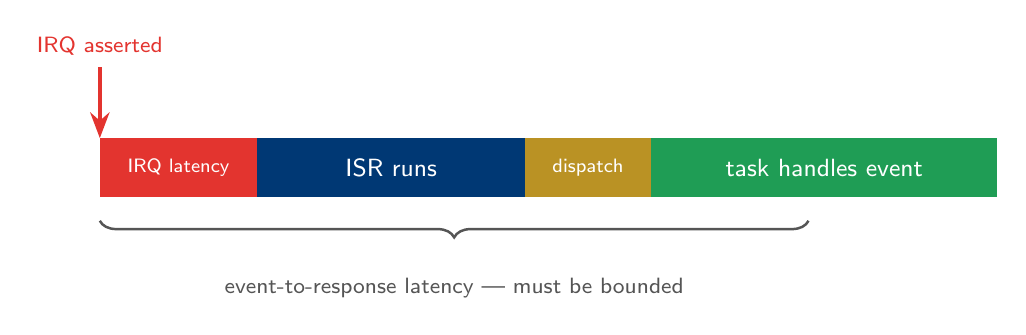
\begin{tikzpicture}[>=Stealth,font=\sffamily,x=1cm,y=1cm]

  % --- bar segments ---
  \fill[rtred]   (0,0)   rectangle (2.0,0.75);
  \fill[kmblue]  (2.0,0) rectangle (5.4,0.75);
  \fill[kmgold]  (5.4,0) rectangle (7.0,0.75);
  \fill[rtgreen] (7.0,0) rectangle (11.4,0.75);

  % --- segment labels ---
  \node[white,font=\sffamily\scriptsize] at (1.0,0.375) {IRQ latency};
  \node[white,font=\sffamily\small]      at (3.7,0.375) {ISR runs};
  \node[white,font=\sffamily\scriptsize] at (6.2,0.375) {dispatch};
  \node[white,font=\sffamily\small]      at (9.2,0.375) {task handles event};

  % --- event arrow ---
  \draw[rtred,line width=1.4pt,->] (0,1.65) -- (0,0.75);
  \node[rtred,font=\sffamily\footnotesize,above] at (0,1.68)
        {IRQ asserted};

  % --- event-to-response brace ---
  \draw[dkgray,line width=0.9pt,decorate,
        decoration={brace,amplitude=6pt,mirror}] (0,-0.3) -- (9.0,-0.3);
  \node[dkgray,font=\sffamily\footnotesize] at (4.5,-1.15)
        {event-to-response latency --- must be bounded};

\end{tikzpicture}
\end{document}
